\documentclass{report}

\usepackage[a4paper, total={170mm,257mm}]{geometry}
% \usepackage{CJKutf8}
\usepackage[utf8]{inputenc}

\usepackage{amsmath}
\usepackage{amsthm}
\usepackage{amssymb}
\usepackage{hyperref}
\usepackage{graphicx}


\newtheorem{theorem}{Theorem}[section]
\newtheorem{corollary}{Corollary}[theorem]
\newtheorem{lemma}[theorem]{Lemma}


\title{%
Selected solutions for past entrance exams \\
\large{dept. of Computer Science, IST, \\
The University of Tokyo}}


\author{Przemek}
\date{January 2020}

\begin{document}

\maketitle

%%%%%%%%%%%%%%%%%%%%%%%%%%%%%%%%%%%%%%%%%%%%%%%%
%%%%%%%%%%%%%%%%%%%%%%%%%%%%%%%%%%%%%%%%%%%%%%%%
\vspace*{\fill}
\begin{center}
Past exams can be found here: \url{http://bit.ly/todai-cs}
\end{center}

\begin{center}
I do not guarantee correctness of the solutions.

\textbf{Use on your own risk.}
\end{center}
\vspace*{\fill}
%%%%%%%%%%%%%%%%%%%%%%%%%%%%%%%%%%%%%%%%%%%%%%%%
%%%%%%%%%%%%%%%%%%%%%%%%%%%%%%%%%%%%%%%%%%%%%%%%

\tableofcontents

\newpage

\chapter{Winter 2019}
\section{Problem 1 – Logic Circuit Design \textit{(send help)}}

\paragraph{Question 1}
\emph{Joint effort.}
Thanks to Igor who first brute-forced the solution for $n=3$.
Takato did the same but using \emph{k-maps} for each $M_i$.

Taku first draw a table for $n=2$:   

\begin{table}[!h]
\centering
\begin{tabular}{cc|cccc}
$K_1$ & $K_0$ & $M_3$ & $M_2$ & $M_1$ & $M_0$ \\
\hline
0  & 0  & 0  & 0 & 0 & 1 \\
0  & 1  & 0  & 0 & 1 & 1 \\
1  & 0  & 0  & 1 & 1 & 1 \\
1  & 1  & 1  & 1 & 1 & 1
\end{tabular}
\end{table}
And then for $n=3$:
\begin{table}[!h]
\centering
\begin{tabular}{lll|llll|llll}
$K_2$ & $K_1$ & $K_0$ & $M_7$ & $M_6$ & $M_5$ & $M_4$ & $M_3$ & $M_2$ & $M_1$ & $M_0$ \\
\hline
0  & 0  & 0  &    &    &    &    &    &    &    & 1  \\
0  & 0  & 1  &    &    &    &    &    &    & 1  & 1  \\
0  & 1  & 0  &    &    &    &    &    & 1  & 1  & 1  \\
0  & 1  & 1  &    &    &    &    & 1  & 1  & 1  & 1  \\
\hline
1  & 0  & 0  &    &    &    & 1  & 1  & 1  & 1  & 1  \\
1  & 0  & 1  &    &    & 1  & 1  & 1  & 1  & 1  & 1  \\
1  & 1  & 0  &    & 1  & 1  & 1  & 1  & 1  & 1  & 1  \\
1  & 1  & 1  & 1  & 1  & 1  & 1  & 1  & 1  & 1  & 1 
\end{tabular}
\end{table}

Notice the repetitive pattern above.
Let's build solution for $n=3$ using $n=2$.
A circuit for $n=2$ is easy to build: let it have inputs $K_1^{(2)}, K_0^{(2)}$ and outputs $M_i^{(2)}$ for $i=0,1,2,3$.
Let the solution for $n=3$ have inputs $K_j^{(3)}$ for $j=0,1,2$ and outputs $M_l^{(3)}$ for $l=0,1,\cdots7$.
Now set:
\begin{align*}
    K_0^{(2)} &:= K_0^{(3)} \\
    K_1^{(2)} &:= K_1^{(3)} \\
    M_i^{(3)} &:= M_i^{(2)} \lor K_2^{(3)}  && \text{for $i=0,1,2,3$} \\
    M_i^{(3)} &:= M_i^{(2)} \land K_2^{(3)}  && \text{for $i=4,5,6,7$}
\end{align*}

This way we can generalize: to build solution for $n+1$, we can reuse solution for $n$ with addition of $2^n$ more gates.
More specifically, solution for $n$ has $2^n$ outputs.
We \emph{or} first 'half' of output wires with $K_{n+1}$, and \emph{and} the rest.

With this recursive definition, we can easily compute $S(n)$ \textit{size} of the circuit with $n$ inputs:
\begin{align*}
    S(n) = S(n-1) + 2^{n} = \sum_{i=0}^{i=n} 2^i = 2^{n+1} - 1 = O(N)
\end{align*}

Let $D(n)$ denote \textit{depth} of the circuit with $n$ inputs. Recall that $N=2^n$ stands for number of outputs.
\begin{align*}
    D(n) = D(n-1) + 1 = O(n) = O(\log N)
\end{align*}

Don't forget to add a switch $Z$ at the end of the final answer:
simply \emph{and} every $M_i$ with negated $Z$.
It adds $1$ to depth and $2^n$ to size.
Although, it doesn't change asymptotic size and depth, respectively.


\paragraph{Question 2}
(send help) Limitation on depth makes it difficult.

\section{Problem 2 – Bucket Sort}

Setting of the problem: we got $N$ element and $K$ buckets.

\paragraph{Question 1}
\begin{verbatim}
B[m].get(j)
\end{verbatim}

\paragraph{Question 2}
The input sequence might be in an \textbf{increasing} order and all elements might fall into one bucket.
Thus, line $6$ will be executed:
\begin{equation*}
    C = 0 + 1 + \cdots + (n-1) = \frac{n(n-1)}{2}
\end{equation*}
times.
Note that it has to be an increasing order, because items are being inserted at the beginning of a bucket.
If we wanna do evil, we must make every item traverse the whole bucket, until the end.
It is possible when every inserted item is bigger than any element in the bucket, that is, input sequence is of increasing order.


\paragraph{Question 3}
Let $n_i$ denote size of $i$-th bucket.
Line $6$ is de facto an \emph{insertion sort}, which means that $i$-th~bucket will be sorted in $O(n^2)$.
Total running time will be  to:
\begin{equation*}
    C = \sum_{i=1}^{K} O(n_i^2)
\end{equation*}
Taking expectation:
\begin{equation*}
    \mathbb{E}(C) = \mathbb{E}[\sum_{i=1}^{K} O(n_i^2)]
                  = \sum_{i=1}^{K} \mathbb{E}[O(n_i^2)]
                  = \sum_{i=1}^{K} O(\mathbb{E}[n_i^2])
\end{equation*}
What is $[\mathbb{E}n_i^2]$? 
Note that, by definition $Var(X) = \mathbb{E}[X^2] - (\mathbb{E}X)^2$ for any random variable $X$.
Let $X_{i,j}$ be an indicator random variable:
\begin{equation*}
    X_{i,j} = \begin{cases}
    1 & \text{element $j$ went to bucket $i$} \\
    0 &  \text{otherwise}
    \end{cases}
\end{equation*}
\begin{equation*}
    n_i = \sum_{j=1}^{N} X_{i, j}
\end{equation*}
Since we have $K$ buckets and every of them is equally likely, probability of "going to bucket $i$" is $\frac{1}{K}$.
Thus, expectation of $n_i$ is:
\begin{equation*}
     \mathbb{E}(n_i) = \sum_{j=1}^{N} \mathbb{E}(X_{i, j}) = \frac{N}{K}
\end{equation*}

We can also notice, that, $n_i$ is just a binomial random variable with expectation $np$ and variance $np(1-p)$.
Here a trial is mapping an item into bucket, and the success is placing it into $i$-th bucket.
There are $n=N$ trials and probability of success if $\frac{1}{K}$.
\begin{align*}
    \mathbb{E}[n_i^2] = Var[n_i] + (\mathbb{E}[n_i])^2 &= N\frac{1}{K}(1-\frac{1}{K}) + (\frac{N}{K})^2 \\
    &= \frac{N^2 + NK - N}{K^2}
\end{align*}
Finally:
\begin{align*}
    \mathbb{E}[C]   = O(\sum_{i=1}^{K}\mathbb{E}[n_i^2]) 
                    = O(\sum_{i=1}^{K} \frac{N^2 + NK - N}{K^2})
                    = O(\frac{N^2}{K} + N)
\end{align*}

\paragraph{Question 3}
The following contribute to total expected running time:
\begin{itemize}
    \item finding a bucket for each element $O(N)$
    \item sorting each bucket, $O(\frac{N^2}{K} + N)$
    \item for each bucket, getting its content: $O(K\frac{N}{K}) = O(N)$
\end{itemize}
Total running time:
\begin{equation*}
    O(\frac{N^2}{K} + 3N)
\end{equation*}
When $K$ is $O(N)$, then we get $O(N)$ expected running time.
When $K$ is $O(1)$, then the running time is $O(N^2)$.

\paragraph{Question 4}
\begin{itemize}
    \item BS is stable, QS isn't
    \item BS isn't in-place, QS is
    \item BS runs $O(N)$ expected, QS is $O(NlogN)$
    \item BS has upper limit on keys, QS hasn't
\end{itemize}




\section{Problem 3 – Automata Theory}
\paragraph{Question 1}
\begin{verbatim}
--> o --a--> o --a--> o --b--> (o)
   / \      / \      / \       / \
   \ /      \ /      \ /       \ /
    E        E        E         E
\end{verbatim}


\paragraph{Question 2}
Write
\begin{equation*}
    L_2 = \{w \in \Sigma^* | v \preceq w \text{ for some } v \in L \}
\end{equation*}
where $v \preceq w$ indicates that $v$ is subsequence of $w$.
In other words, to in order to get a word from $L_2$, we first fix a word $v \in L$ and then intertwine its letters with some "garbage" from $\Sigma^*$.

% The first idea is to reuse Q1: for each $v \in L$, $v = v_1 v_2\cdots v_{|v|}$ we will create a "small" automaton with $v_{|v|}$ states.
% We will label transitions between next states with $v_1, v_2, \cdots, v_{|n|}$.
% Additionally, each state has a loop to itself labeled with $\Sigma^*$. 
% The last state (with incoming edge $v_{|v|}$) is an accepting state.
% The "big" automaton $A_2$ which accepts $L_2$ consists of $|L|$ "small" automatons.
% First states in every "small" automaton (i.e with edge $v_1$) make set of starting state of $A_2$.

Let's fix $v\in L$.
Let $p_1, p_2, \cdots p_{|v|}$ be sequence of states that $\mathcal{A}$ visits when reading $v$.
Label transitions between $p_i$'s with next letters of $v$.
Moreover, for each $p_i$, add a loop to itself labeled with $\Sigma$.
Make $p_1$ the start state.

\paragraph{Question 3}
First,
\begin{equation*}
    L' = \{ w \in \Sigma^* | v\in L \text{ for every } v\in \Sigma^* \text{ such that  } v\preceq w\}
\end{equation*}
is kinda quirky. 
We already supposed that $L \subseteq \Sigma^*$, so why do we need $v\in \Sigma^*$ above?

Let's start with constructing a NFA $\mathcal{N}$ which accepts L'.
Let $\mathcal{N}$ be a copy of $\mathcal{A}$, where we additionally put $\Sigma$-labeled loops on every state.
Intuitively, while traversing $\mathcal{A}$, in every state, we can have a "detour", i.e. accept some garbage.

Having constructed NFA $\mathcal{N}$, move to constructing equivalent DFA $\mathcal{D}$.
It is feasible, and subset construction tells us how to it.
Formally, define automaton $\mathcal{A}$ accepting $L$ as $\mathcal{A} = (Q, \Sigma, \delta, q_o, F)$.
NFA $\mathcal{N}$ such that $\mathcal{L}(\mathcal{N}) = L'$ is defined as:
\begin{align*}
    \mathcal{N} &= (Q, \Sigma, \delta_N, q_0, F)
\end{align*}
where
\begin{equation*}
    \delta_N(q, a) = \{q\} \cup \{\delta(q,a)\}
\end{equation*}
is a "loop" on every state.
Now, equivalent DFA $\mathcal{D}$ is obtained by subset construction:
\begin{align*}
    \mathcal{D} &= (Q_D, \Sigma, \delta_D, {q_0}, F_D) \\
    Q_D &= \mathcal{P}(Q) \\
    F_D &= \{ X\in Q_D | X\cap F \neq \emptyset\} \\
    \delta_D(X,a) &= \bigcup_{q \in X} \delta_N(q,a)
\end{align*}


\paragraph{Question 4}
Since every DFA has equivalent NFA and vice versa, I'll prove (Q3) for NFA $\mathcal{N}$.
Two steps:
\begin{itemize}
    \item $w \in L' \Rightarrow \mathcal{N} \text{ accepts } w$.
    Since $w\in L'$, then there must exits $v\in L$ such that $v\preceq w$.
    $v$ is accepted both in $\mathcal{A}$ and $\mathcal{N}$, since $\mathcal{N}$ has exactly the same states as $\mathcal{A}$.
    Then, $w$ must be accepted by $\mathcal{N}$ by following the loops on letters of $w$ which do not contribute to $v$.
    \item $\mathcal{N} \text{ accepts } w \Rightarrow w \in L'$.
    To get $v$ such that $v\preceq w$, simulate $\mathcal{N}$ on $w$, skip the loops. 
    Obviously $v\in L$, because states of $\mathcal{N}$ and $\mathcal{A}$ are the same and $v$ and $w$ will end up in the same final state of $\mathcal{N}$.
\end{itemize}



\section{Problem 4 – Linear Algebra}

\paragraph{Question 1}
Condition number $\kappa(A)$ of $A$ is:
\begin{equation*}
    \kappa(A) = ||A|| \: ||A^{-1}||
\end{equation*}
where $||\cdot ||$ denotes a norm of a matrix:
\begin{equation*}
    ||A|| = \max_{x\in \mathbb{R^N}} \frac{||Ax||}{||x||} = \max_{x: ||x||=1} ||Ax||
\end{equation*}



\paragraph{Question 2}
Not sure if OK...  \\ We know $Ax = b$ and let $r = b- A\hat{x}$:
\begin{align*}
    (A+E)\hat{x} &= b \\
    A\hat{x} + E\hat{x} &= b \\
    E\hat{x} &= b - A\hat{x} \\
    E\hat{x} &= r
\end{align*}
But how do we know if $E$ is rank $1$?


\paragraph{Question 3}
\begin{align*}
    (A+ \delta A)(x+ \delta x) = b \\
    Ax + A(\delta x) + \delta A(x+ \delta x) = b
\end{align*}
Substituting $Ax = b$:
\begin{align*}
    A(\delta x) + \delta A(x+ \delta x) &= 0 \\
    - A(\delta x) &= \delta A(x+ \delta x) \\
    -\delta x &= A^{-1} (\delta A)(x+ \delta x)
\end{align*}
because matrix $A$ is not singular, so inverse $A^{-1}$ exist.
Now, take the norm both sides.
We are assuming that $A + \sigma A$ is not singular, so it has inverse and thus a norm:
\begin{align*}
    ||\delta x || &= || A^{-1} \: [\delta A(x+ \delta x) ]|| \\
      &\leq || A^{-1} ||  \: || \delta A(x+ \delta x) || \\
      &\leq || A^{-1} ||  \: || \delta A || \: || x + \delta x ||
\end{align*}
\begin{align*}
    \frac{||\delta x ||}{ || x + \delta x || } &\leq || A^{-1} ||  \: || \delta A || \\
    &= || A^{-1} || \:  \frac{|| A^{1} || }{|| A^{1} ||} || \delta A || \\
    &= \kappa(A) \frac{||\delta A||}{||A||}
\end{align*}

\paragraph{Question 4}
When an $n$ dimensional real matrix C is singular, there is a non-zero, real vector $y$ such that $Cy = 0$. 
\textit{In particular}, we can choose a unit vector $y' = \frac{y}{||y||}$. 

Let $x \in nullspace(B)$ be a unit vector i.e. $Bx = 0$ and $||x|| = 1$.
\begin{align*}
    ||A-B|| &= ||A-B|| \: ||x|| \\
            &\geq || (A-B)x || \\
            &= ||Ax - Bx|| \\
            &= ||Ax||
\end{align*}
On the other hand:
\begin{align*}
    1 = ||x|| = || A^{-1} \:(Ax) || &\leq || A^{-1} || \: ||Ax|| \\
    ||Ax|| &\geq \frac{1}{||A^{-1}||}
\end{align*}
More on condition numbers:\newline
\url{https://blogs.mathworks.com/cleve/2017/07/17/what-is-the-condition-number-of-a-matrix/}.

\chapter{Winter 2018}
\section{Problem 1 – Linear Algebra}

\paragraph{Question 1}
Let $x$ be an eigenvector with corresponding eigenvalue $\lambda$: $Ax = \lambda x$.
Let $\mu \in \mathbb{R}$. 
\begin{equation*}
    (A + \mu I)x = Ax + \mu x = \lambda x + \mu x = (\lambda + \mu)x
\end{equation*}
So $x$ is an eigenvector of $(A + \mu I)$ with corresponding eigenvalue of $\lambda + \mu$.


\paragraph{Question 2}
Let $v \in \mathbb{R^N}$ be a unit vector which maximizes $v^T A v$.
Because $A$ is real and symmetric, then it can be diagonalized $A = Q^T \Lambda Q$, where $Q$ is orthogonal matrix, which columns form orthogonal basis.
In following equation, let's substitute $y = Qv$:
\begin{align*}
    v^T A v &= v^T Q^T \Lambda Q v = y^T \Lambda y \\
            &= \sum_{i=1}^{N}\lambda_i y_i^2\\
            &\leq \: \sum_{i=1}^{N} \lambda_{max}(A) \: y_i^2
              = \lambda_{max}(A) \: \sum_{i=1}^{N} y_i^2\\
            &= \lambda_{max}(A) \: y^T y = \lambda_{max}(A) \: v^T Q^T Q v\\
            &= \lambda_{max}(A)
\end{align*}
On the other hand, let $x_{max}$ be eigenvector corresponding to $\lambda_{max}(A)$.
Because $v$ maximizes $v^T A v$, then:
\begin{equation*}
    v^T A v \geq x_{max}^T (A x_{max} ) = x_{max}^T  x_{max} \: \lambda_{max}(A)  = \lambda_{max}(A)
\end{equation*}
Here we got:
\begin{equation*}
    \lambda_{max}(A) \leq v^T A v \leq \lambda_{max}(A)
\end{equation*}
For vector $v$ which maximizes $v^T A v$.
Hence,
\begin{equation*}
    \lambda_{max}(A) = \max \{v^T A v | v\in\mathbb{R}^N, v^T v = 1\}
\end{equation*}
and the maximum is reached for eigenvector $x_{max}$.

\paragraph{Question 2}
 Let $v\in\mathbb{R}^N$.
From question (2) we know that $v^T A v\leq \lambda_{max}(A) v^T v$ for arbitrary $v$: look at second to the last line of Q2 calculations.
Now if we know that fact, we get the inequality trivially:

\begin{align*}
    v^T(\lambda_{max}(A) I - A) v 
        = \lambda_{max}(A) v^T v - v^T A v
        \geq 0
\end{align*}


\paragraph{Question 3}
Since $A, B$ are symmetric and real, then $A = Q^T\Lambda_A Q$ and $B = P^T\Lambda_B P$ for some orthogonal $Q$~and~$P$.
From what we obtained in (Q2): let $w$ be a~unit vector which maximizes $w^T(A+B)w$.
Then:
\begin{align*}
    \Lambda_{max}(A+B) &= w^T(A+B)w \\
                        &= w^T A w + w^T B w \\
                        &= w^T Q^T \Lambda_A Q w + w^T P^T \Lambda_B P w = (*)
\end{align*} 
Substitute $y = Qw$ and $z = Pw$. Of course $y^T y = z^T z = 1$, because $y^T y = w^TQ^TQw = w^T w = 1$ (the same for $z$).
Combining this and our knowledge form previous questions:
\begin{align*}
    (*) &= y^T \Lambda_A y + z^T \Lambda_B z \\
            &\leq \lambda_{max}(A) \: y^T y + \lambda_{max}(B) \: z^T z \\
            &= \lambda_{max}(A) + \lambda_{max}(B)
\end{align*}


\section{Problem 2 – Automata theory}
\paragraph{Question 1}
\emph{This one was also solved in \textbf{Automata Theory, Languages and computation 3rd ed}, 2.2.4, Example 2.4}
\begin{figure}[!h]
    \centering
    \includegraphics[scale=0.3]{data/2018-W-2-1.png}
    \caption{Question 1.}
\end{figure}



Explanation:
\begin{itemize}
    \item A – "number of $a$'s is \textbf{even}, number of $b$'s is \textbf{even}"
    \item B – "number of $a$'s is \textbf{odd}, number of $b$'s is \textbf{even}"
    \item C – "number of $a$'s is \textbf{even}, number of $b$'s is \textbf{odd}"
    \item D – "number of $a$'s is \textbf{odd}, number of $b$'s is \textbf{odd}"
\end{itemize}


\paragraph{Question 2}
Begin with an $\epsilon$-NFA as depiced in Fig. \ref{fig:w1822a}.
It "guesses" which letter appears even number of times.
To make it $\epsilon$-free, we either follow him: \url{https://youtu.be/sq-dLKAd6bo?t=1714} or consider the followig:
starting from start state, how far, i.e. which states can we reach on letter $a$?
There are $3$ such states.
We simply draw an edge to those states.
Do the same for $b,c$. 
The final answer is on Fig. \ref{fig:w1822b}
\begin{figure}[!h]
    \centering
    \includegraphics[scale=0.3]{data/2018-W-2-2a.png}
    \caption{Question 2.  $\epsilon$-NFA.}
    \label{fig:w1822a}
\end{figure}
\begin{figure}[!h]
    \centering
    \includegraphics[scale=0.3]{data/2018-W-2-2b.png}
    \caption{Question 2. $\epsilon$-free NFA. We followed former $\epsilon$-transitions and added new edges (in blue). Thanks Taku!}
    \label{fig:w1822b}
\end{figure}




\paragraph{Question 3}
\emph{Prove that, for every $n\geq 1$, every \textbf{deterministic} finite state automaton that accepts $L_{\exists ,n}$ has at least $2^n$ states.}

\emph{First, I'll show that there is a DFA with $2^n$ states.}
We can encode states of DFA $L_{\exists ,n}$ as a binary string $B = (b_n, b_{n-1}, \cdots, b_2, b_1)$ of length $n$, where $b_i = 1$ iff numbers of $a_i$'s is odd in so-far read sequence, else $0$.
A state is accepting if its binary representation has at least one zero.
There are $2^n$ such strings.

\emph{Now, I'll show that there is no DFA with less than $2^n$ states.}
If the DFA had fewer than $2^n$ states, then there would be some state $q$ such that the DFA can be in state $q$ after reading two different sequences of length $n$, say $a = a_1a_2\cdots a_n$ and $b = b_1b_2\cdots b_n$.
If the sequences were of \emph{different parity}, i.e. one of the sequences had a letter which appears even number of times, and the other sequence hadn't, then $q$ would be both accepting and nonaccepting state.
If the sequences were of the same parity, then we could append some sequence $c_1\cdots c_m \in \Sigma^*$ to $a$ and $b$ such that $a_1a_2\cdots a_n c_1\cdots c_m$ and $b_1b_2\cdots b_n c_1\cdots c_m$ have different parity.
Consider state $p$ that the DFA enters after reading $c_1\cdots c_m$. 
Then $p$ must be both accepting and nonaccepting, since either of
$a_1a_2\cdots a_n c_1\cdots c_m$ and $b_1b_2\cdots b_n c_1\cdots c_m$ is accepted and the other isn't.

This problem could be also one-lined using \textit{Myhill-Nerode theorem}.
The only one difficulty here is to define $2^n$ equivalent classes.
Try fiddling with binary strings.



\paragraph{Question 4}
\emph{Prove that, for every $n\geq 1$, every \textbf{non-deterministic} finite state automaton (without $\epsilon$-transitions) that accepts $L_{\forall ,n}$ has at least $2^n$ states.}
Begin with constructing DFA $A$ accepting $L_{\forall ,n}$ the same way as in Q3 – except that $A$ has only one accepting state, a string of all $0$'s.
Obviously this DFA is also a~NFA.
The equivalent NFA simply cannot \textit{guess} parity of some letters: it has to remember information of parity of each letter.
As shown in Q3, every letter requires $2$ bits, so minimum of $2^n$ states are required.

\emph{s e n d h e l p}




\section{Problem 3 – Union-Find}
\emph{See chapter $21$ of Cormen (3rd edition) for more.}

We have set of $2^N$ elements. 
\emph{MERGE}($A, B$) changes $A$'s root's pointer so that it points root of $B$.

\paragraph{Question 1}
$2^N-1$ merge operations are required to merge all the subsets.

\paragraph{Question 2}
Minimum tree height: $1$ – one root with $2^N - 1$ leafs. 
How to: Fix root $r$ and perform \emph{MERGE}($v, r$) for every other element $v \neq r$.

\paragraph{Question 3}
Maximum tree height: $2^N -1$.
How to: start with a tree consisting of one element.
While merging the tree and a node, make the tree point the node.
In pseudo-code: 
\begin{verbatim}
for i in range(1, 2**N):
    merge(v[i-1], v[i])
\end{verbatim}


\paragraph{Question 4}
New MERGE(A, B): change pointer of the root node of subset with smaller height so that it points to root node of the other subset. 
This technique is called \emph{merge (union) by rank} (rank - upper bound on the height of the node).
How to get a tree with maximum height?
The observation is, merging trees having the same height will result in a taller tree.
If $A$ and $B$ have height of $h$, then merged tree is of height $h+1$.

Suppose we had a maximum-height tree with $2^N$ nodes.
It must have been obtained by merging of two maximum-height trees with $2^{N-1}$ nodes.
\begin{equation*}
    H(2^N) = 1 + H(2^{N-1}) = N
\end{equation*}


\paragraph{Question 4}
During execution of FIND, we make every node on the find-path point directly to the root.
This technique is called \emph{path compression}.

In details, first we find a path from a node its root. 
Then, we go through the path again and change pointers of nodes on the path.
Original FIND was linear in length of the path.
Now we scan the path twice, which still yields linear time.



\section{Problem 4 –  Synchronization}

\paragraph{Question 1}
Its $1$ and $2$.
On a sequential execution we get $2$.
We can get $1$ when one process loads a value before another process stores it.

\paragraph{Question 2}
Test-and-set writes $1$ to memory and returns previously stored value.

\begin{verbatim}
int TestAndSet(int *a) {
    int b;
    b = *a;
    *a = 1;
    return b;
}
\end{verbatim}


\paragraph{Question 3}
Swap:
\begin{verbatim}
void Swap(int *a, int *b) {
    int tmp = *a;
    *a = *b;
    *b = tmp;
}
\end{verbatim}
Answer:
\begin{verbatim}
int key = 1;
while (key == 1)
    Swap(&key, &lock);
x = x + 1;
lock = 0;
\end{verbatim}



\chapter{Winter 2017}
\section{Problem 1 – Linear Algebra}
\paragraph{Question 1}
\begin{equation*}
  ||x||_2 = \sqrt{\sum_{i=1}^{n} x_{i}^2} \leq \sum_{i=1}^{n} \sqrt{x_{i}^2}
 = \sum_{i=1}^{n} |x_{i}| = ||x||_{1}  
\end{equation*}

On the other hand, let $y\in \mathbb{R}^n$ be a unit vector:
\begin{align*}
   ||x||_1 = | x \cdot y | &\leq ||x||_{2} ||y||_{2} \\
   &= ||x||_{2} \sqrt{1+1+\dots+1}  \\
   &= \sqrt{n}  ||x||_{2}
\end{align*}
The first inequality comes from Cauchy-Schwarz inequality: $|xy| \leq ||x||_2 ||y||_2$.

\paragraph{Question 2.1}
Matrix $A$ defines some transformation and $||A||_p$ measures how original vector will be stretched by the transformation.
If $||A||_p < 1$ then the transformation \textit{shrinks} the vector.
By applying the transformation multiple times, we will shrink the vector more and more.
In particular, applying it infinitely many times will shrink the vector to zero.
Formally:
\begin{align*}
0 &\leq \lim_{k \to \infty} ||A^k x_0||_p \\
      &\leq \lim_{k \to \infty} ||A^k||_p || x_0||_p \\
      &=  || x_0||_p \lim_{k \to \infty} ||A^k||_p  \\
      &=  || x_0||_p \: 0 \\
      &= 0
\end{align*}
First equality holds because norm is always non-negative,
second is a property of a norm. 
Moreover, limit $\lim_{k \to \infty} ||A^k||_p = 0$, because:
\begin{equation*}
    \lim_{k \to \infty} ||A^k||_p \leq \lim_{k \to \infty} (||A||_p)^k =0
\end{equation*}
NB: $||AB||_p \leq ||A||_p ||B||_p$ for any matrices $A,B \in \mathbb{R}^{n\times n}$.

\paragraph{Question 2.2}
Since $A$ is symmetric, then it can be diagonalized $A=Q^T\Lambda Q$, where $Q$ is orthogonal matrix (i.e. $Q^T Q = I $).
Note that 
\begin{equation*}
    \max_{x} \frac{||Ax||_p}{||x||_p} = \max_{x: ||x||_p = 1} ||Ax||_p
\end{equation*}
Let $x$ be a unit vector which maximizes the above.
We have:
\begin{align*}
    ||Ax||_2 &= (Ax)^T (Ax) \\
            &= x^T Q^T \Lambda Q Q^T \Lambda Q x \\
            &= x^T Q^T \Lambda^2 Q x
\end{align*}
By substituting $y = Qx$:
\begin{align*}
    ||Ax||_2 &= y^T \Lambda^2 y \\
            &= \sum \lambda_i^2 y_i^2 \\
            &\leq \sum \lambda_{max} y_i^2  \\
            &=\lambda_{max} \sum  y_i^2  \\
            &= \lambda_{max} \: y^T  y \\
            &= \lambda_{max}
\end{align*}
Because $y^T y = (Qx)^T(Qx) = x^T Q^T Q x = x^T x = 1$.
On the other hand, let $q$ be eigenvector corresponding to $\lambda_{max}$.
Of course $||q||_2 =1$, because $Q$ is orthogonal.
\begin{align*}
    ||Aq||_2 &\geq ||Aq||_2 \\
            &= ||\lambda_{max} q ||_2 \\
            &= \lambda_{max} ||q||_2 \\
            &= \lambda_{max}
\end{align*}




\paragraph{Question 3}
Let $e^{(j)} = x^{(j)} - x$ be the error vector. 
We want $\lim_{j\to \infty} e^{(j)} = 0$.
In other words, we want $e^{(j+1)} < e^{(j)}$ for all sufficiently \textit{big} $j$.
% Let's subtract $x$ from original equation:
\begin{align*}
e^{(j+1)} = x^{(j+1)} - x &=  b - x  + (I -A) x^{(j)}  \\
                &= Ax - x  + (I -A) x^{(j)}  \\
                &= -(I-A)x  + (I -A) x^{(j)}  \\
                &= (I -A)(x^{(j)} - x) \\
\end{align*}
Here, we obtain: $e^{(j+1)} = (I -A) e^{(j)}$. 
Taking a norm both sides:
\begin{align*}
    ||e^{(j+1)}|| &= ||(I -A) e^{(j)}|| \\
              &\leq ||I -A|| \: || e^{(j)}||
\end{align*}
Thus, the sequence converge to real solution if 
\begin{equation*}
    ||I -A|| < 1
\end{equation*}

More reading:
\url{http://runge.math.smu.edu/Courses/Math3315_Spring10/iterative_linear.pdf}


\section{Problem 2 – Automata Theory}

\paragraph{Question 1}
$x = a$, $y = bc$ and $z = c$

\paragraph{Question 2}
Classic proof of Pumping Lemma (PL) for regular languages.
Let $\mathcal{M}$ be an automaton with $k$ states.
Let $w = a_1a_2\cdots a_k \in L(M)$ such that $|w| > k$.
Now let's simulate run of $\mathcal{M}$ of word $w$.
Define states $p_i = \hat\delta(q_0, w_1w_2\cdots w_i)$.
That is, $p_i$ is a state in which $\mathcal{M}$ is after reading first $i$ inputs.
From pigeonhole principle, at lest two of those state must be exactly the same state.
Let $p_i = p_j$ be the state that is visited the second time for the first time (i.e. $i$ is the smallest among all such states).

I claim that: $w = xyz$, where 
\begin{itemize}
    \item $x = a_1a_2\cdots a_{i-1}$
    \item $y = a_ia_{i+1}\cdots a_{j-1}$
    \item $z = a_ja_{j+1}\cdots a_k$
\end{itemize}
Obviously, $|y| > 0$ because $i\neq j$ and $|xy| = j - 1 \leq n$.
States $p_i, \dots, p_j$ create a loop in the automaton - it can be traversed any number of times, thus $xy^nz \in L(\mathcal{M})$.
For $n=0$ we simply "skip" the loop, for $n\geq 1$ we traverse the loop $n$ times.


\paragraph{Question 3}
$L(M) = \{ a^m b^n | n,m \in \mathbb{N}, 0<m<n \}$
Assume that $L$ is regular language.
Then pumping lemma must hold.
Consider $w = a^k b^{k+1} \in L $, where $k$ is the pumping lemma constant.
Because $|w| = 2k + 1 > k$, then there must exist a partitioning
$xyz = w$ such that $|xy| < k$, $|y|>0$ and $xy^nz \in L$ \textbf{for all} $n\in\mathbb{N}$.
Notice that $xy$ consists of $a$'s only.
Let's "pump up" $y$.
For example, $xy^{42}z$ contains of significantly more $a$'s than $b$'s.
This word does not belong to the language.
Contradiction with statement that $x y^n z \in L$ for all $n\in N$.
$L(M)$ is not regular, thus there exist no automaton recognizing it.


\section{Problem 3 – Heapsort}

\paragraph{Question 1}
\begin{enumerate}
    \item Building the heap – level-by-level, starting from the deepest level.
    \item Extracting minimum $n$ times. Extracting means printing the root value, replacing it with the last heap element, and then fixing heap order. 
    If we represent the heap in an array of length $n$, we can swap first element (minimum) with the last element, fix heap order and call recursively on first $n-1$ elements of array.
    Resulting array is sorted in descending order.
    Reverse it for ascending order.
\end{enumerate}

\paragraph{Question 2}
Let's put elements of $[3,8,1,5,4,9,7]$ into a binary tree:
\begin{verbatim}
        3
      /    \
     8      1
   /  \    /  \
  5    4  9    7         ] proper heaps
\end{verbatim}
Note that the deepest level consists of $4$ proper, one-element heaps.
Let's fix the heap order on second to last deepest level:
\begin{verbatim}
        3
      /    \
     4      1             ] 
   /  \    /  \           ] proper heaps
  5    8  9    7          ] 
\end{verbatim}
Now we have two proper heaps of height $1$.
Now, swap $3$ and $1$ to get the final answer:
\begin{verbatim}
        1
      /    \
     4      3
   /  \    /  \
  5    8  9    7
\end{verbatim}

\paragraph{Question 3}
For simplicity, assume that $n=2^k - 1$, i.e. the heap the deepest level is fully occupied.

Phase 1, building the heap is $O(n)$ when building the heap from the bottom.
On the deepest level we do nothing: it consists of $\lceil \frac{n}{2} \rceil$ nodes, each of them is a proper one-element heap.
On second-to-the-last level, we perform two comparisons, and possibly one swap.
In general we'll perform, ceil omitted for simplicity:
\begin{align*}
    0\cdot \frac{n}{2} + 1 \cdot \frac{n}{4} + 2\cdot \frac{n}{8} + \cdots + O(h-1)\cdot 2 + O(h)\cdot 1 &= 
    \sum_{h=1}^{\lceil \text{log}_2 n \rceil} \lceil\frac{n}{2^{h+1}}\rceil\cdot O(h) 
    = O(n\sum_{h=1}^{\lceil \text{log}_2 n\rceil} \frac{h}{2^{h+1}})
\end{align*}
Now, let's evaluate the right-hand side:
\begin{align*}
    n\sum_{h=1}^{\lceil \text{log}_2 n\rceil} \frac{h}{2^{h+1}} 
    &\leq \frac{n}{4} \sum_{h=1}^{\infty} \frac{h}{2^{h-1}} && \text{substitute $x=\frac{1}{2}$} \\
    &= \frac{n}{4} \sum_{h=1}^{\infty} hx^{h-1} \\
    &= \frac{n}{4} \frac{d}{dx} \sum_{h=1}^{\infty} x^h\\
    &= \frac{n}{4} \frac{d}{dx} \frac{x}{1-x} \\
    &= \frac{n}{4} \frac{1}{(1-x)^2} \\
    &= \frac{n}{4} \cdot 4 = n
\end{align*}
Thus, we can bound the running time as:
\begin{align*}
    O(n\sum_{h=1}^{\lceil \text{log}_2 n\rceil} \frac{h}{2^{h+1}}) = O(n)
\end{align*}
See Cormen's \emph{Introduction to Algorithms, 3rd ed, Chapter 6.3} for more.

Phase 2 is $O(n\text{log}_2n)$: for each element out of $n$ we perform extract-min, which takes $O(log_2n)$.

\textit{Bonus}: heapsort pseudocode:
\begin{verbatim}
heapsort(T[1..n])
    build-heap(T[1..n])
    for i = n..2
        swap(T[1], T[i])
        shift-down(T[1..(i-1)], 1)
\end{verbatim}


\paragraph{Question 4}
$O(n+k \text{log}_2 n)$.
First, we build heap in $O(n)$, then we perform ext tract-min $k$ times.


\paragraph{Question 5}
Let's look at an example.
If input array is already sorted, then mergesort will just scan through the array with no swaps.
Same with partition in quicksort.
On the other hand heapsort, after building a heap ($O(n)$), will extract minimum and replace it with the last element of array – which is maximum.
The maximum will be later "bubbled" down back to the deepest level.
This means two comparisons and a swap at every of $O(\text{log}_2 n$ iterations.
This is pricey.

The other reason might be caching.
In heapsort, accessing a parent might result in memory accesses which are distant more than $\lceil \frac{n}{2}\rceil$ (in particular leaves' parents).
If $n$ is big, we might have a lot of cache misses.


\section{Problem 4 – Logic Circuit Design}

\paragraph{Question 1}
$a \veebar b = (a \land \lnot b) \lor (\lnot a \land b) $

\paragraph{Question 2}
I'm not quite sure. 
What happens when both clock and input go $1$?
See Fig. \ref{fig:w17-4-2}
\begin{figure}[!h]
    \centering
    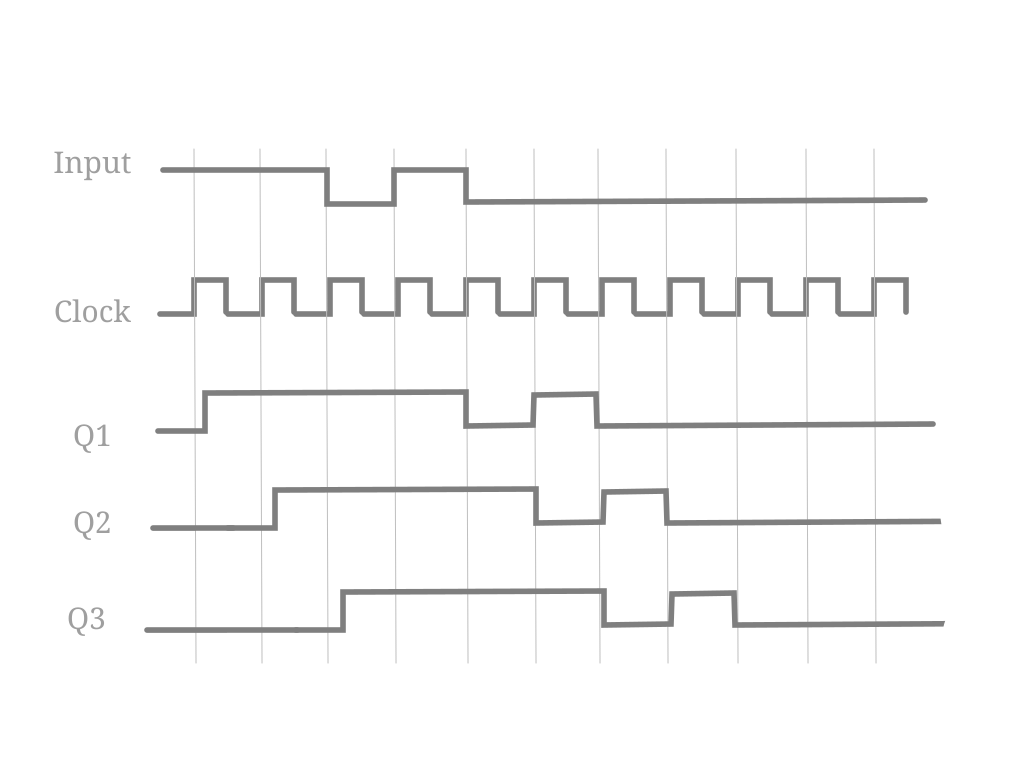
\includegraphics[scale=0.25]{data/2017-W-4-2.png}
    \caption{Question 2}
    \label{fig:w17-4-2}
\end{figure}

\paragraph{Question 3}
See Fig. \ref{fig:w17-4-3}. 
We can construct $xor_{256}$ using $8$ 2-input xors ("binary tree").
\begin{figure}[!h]
    \centering
    \includegraphics[scale=0.25]{data/2017-W-4-3.png}
    \caption{Question 3}
    \label{fig:w17-4-3}
\end{figure}


Give $C_1$ input $C_0$. 
For $i>1$, $C_i$ takes $C_{i-1}$'s output as an input.
Additionally, we \emph{AND} clock signal with negated $W$ and provide it to every $C_i$.

We only modify $X_1$'s input: it takes output of a 2:1 mutex with inputs $X_0$ (0) and the original $xor_{256}$ value (1).
See Fig. \ref{fig:w17-4-4}
\begin{figure}[!h]
    \centering
    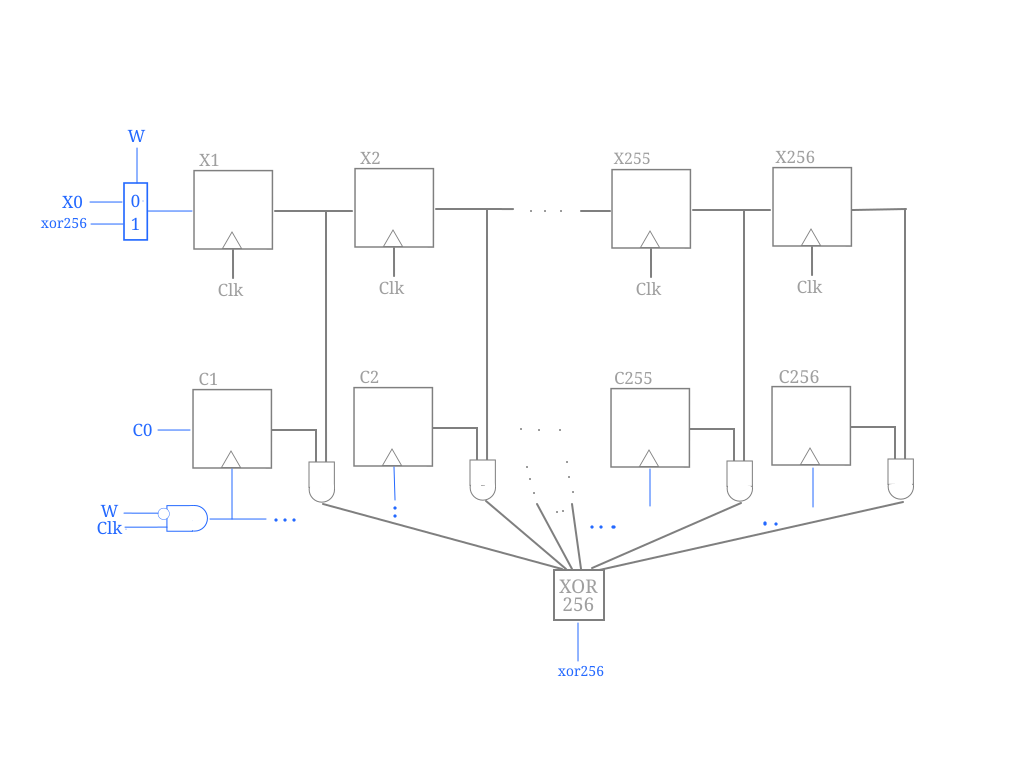
\includegraphics[scale=0.25]{data/2017-W-4-4.png}
    \caption{Question 4. Changes marked blue}
    \label{fig:w17-4-4}
\end{figure}




\chapter{Winter 2016}
\section{Problem 1 – Linear Algebra – LU decomposition}

\paragraph{Question 1}
A lower triangular matrix $M$ has $M_{i,j} = 0$ for $i < j$.
Let $L, L' \in \mathbb{R}^{n\times n}$ be a lower triangular matrices.
Let's look closer at entries above diagonal of $LL'$, i.e. $(LL')_{i,j}$ for $i<j$:
\begin{equation*}
    (LL')_{i,j} = \sum_{k=1}^{n} L_{i,k} \cdot L'_{k,j}
\end{equation*}
Every item of the summation yields either $i<k$ or $k<j$.
Thus,  $(LL')_{i,j} = 0$ for $i<j$.

The same another way:
\begin{align*}
    (LL')_{i,j} &= \sum_{k=1}^{n} L_{i,k} \cdot L'_{k,j} \\
                &= \sum_{k=1}^{j-1} L_{i,k} \cdot L'_{k,j} + \sum_{k=j}^{n} L_{i,k} \cdot L'_{k,j} \\
                &= \sum_{k=1}^{j-1} L_{i,k} \cdot 0 + \sum_{k=j}^{n} 0 \cdot L'_{k,j} \\
                &= 0
\end{align*}


\paragraph{Question 2}
Let $L, L' \in \mathbb{R}^{n\times n}$ be a \emph{unit} lower triangular matrices, i.e $L_{i,j} = L'_{i,j} = 1$ for $i = j$.
We know from Q1, that $LL'$ is lower triangular.
Let's examine diagonal items, $(LL')_{i,i}$:
\begin{equation*}
    (LL')_{i,i} = \sum_{k=1}^{n} L_{i,k} \cdot L'_{k,i}
            = L_{i,1} L'_{1,i} + L_{i,2} L'_{1,i} + \dots + L_{i,i} L'_{i,i} + \dots + L_{i,n} L'_{n,i} = 1
\end{equation*}


\paragraph{Question 3}
Inverse of a unit lower triangular matrix is also unit lower triangular.
So, we need to find only one entry of the inverse of $L1$, such that:
\begin{equation*}
L_1 L_1^{-1} =
\begin{pmatrix}
1 & 0\\
2 & 1
\end{pmatrix}
\cdot
\begin{pmatrix}
1 & 0\\
x & 1
\end{pmatrix}
=
\begin{pmatrix}
1 & 0 \\
0 & 1
\end{pmatrix}
\end{equation*}
Obviously, $x=-2$. Simillary, $L_2$:
\begin{equation*}
L_2 L_2^{-1} =
\begin{pmatrix}
1 & 0 & 0 \\
2 & 1 & 0 \\
3 & 2 & 1
\end{pmatrix}
\cdot
\begin{pmatrix}
1 & 0 & 0 \\
a & 1 & 0 \\
b & c & 1
\end{pmatrix}
=
\begin{pmatrix}
1 & 0 & 0 \\
0 & 1 & 0 \\
0 & 0 & 1
\end{pmatrix}
\end{equation*}
Here, $a = -2$, $b = 1$, $c = -2$.

\paragraph{Question 4}
% Prove that $LU$ decomposition of a matrix is unique if $L$ is \emph{unit} lower triangular matrix.
Prove that if $A$ has two different LU decomposition, that is $A = LU = L_1U_1$ and $L, L_1$ are lower \emph{unit} matrices, then $L=L_1$ and $U=U_1$.

Assume that inverses of $U, U_1$ exist.
Start with $A= LU = L_1 U_1 = A$ and multiply right-hand by $U^{-1}$ and left-hand by $L_1^{-1}$:
\begin{align*}
    LU &= L_1 U_1 \\
    L_1^{-1} L U U^{-1} &= L_1^{-1} L_1 U_1 U^{-1} \\
    L_1^{-1} L  &=  U_1 U^{-1} \\
\end{align*}
We know from (Q2) that left-hand side of the last equation is lower unit triangular matrix.
In similar manner, we can show that right-hand is upper triangular.
Lower and upper triangular matrices can be equal iff they are both diagonal.
Moreover, since $L_1^{-1} L$ has ones on diagonal, so $U_1 U^{-1}$ must have.
We conclude:
\begin{align*}
     L_1^{-1} L = Id = U_1 U^{-1}
\end{align*}
That is, $L = L_1$ and $U = U_1$.
 

\section{Problem 2 – Automata Theory}
\paragraph{Question 1}
$a^*b^*a^*$

\paragraph{Questions 2 - 5}
See Fig. \ref{fig:w2016-w-2-2} - \ref{fig:w2016-w-2-5}

\begin{figure}[!h]
    \centering
    \includegraphics[scale=0.5]{data/2016-W-2-2.png}
    \caption{Question 2}
    \label{fig:w2016-w-2-2}
\end{figure}

\begin{figure}[!h]
    \centering
    \includegraphics[scale=0.5]{data/2016-W-2-3.png}
    \caption{Question 3}
    \label{fig:w2016-w-2-3}
\end{figure}

\begin{figure}[!h]
    \centering
    \includegraphics[scale=0.5]{data/2016-W-2-4.png}
    \caption{Question 4. One of the boxes should be labeled $M_1$.}
       \label{fig:w2016-w-2-4}
\end{figure}

\begin{figure}[!h]
    \centering
    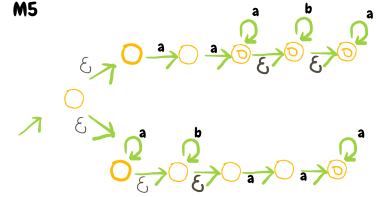
\includegraphics[scale=0.5]{data/2016-W-2-5.png}
    \caption{Question 5. $L(M_5)$ contains $aa$ and is of form of $aaa^* b^* a^* + a^* b^* aaa^*$}
       \label{fig:w2016-w-2-5}
\end{figure}



\section{Problem 3 – AVL Tree}

\paragraph{Question 1}
Easy  % tikz hf

\paragraph{Question 2}
Minimum height of BST with $n$ nodes is $\lfloor log_2n\rfloor$.
Maximum height: $n-1$.

\paragraph{Question 3}
AVL tree with $7$ nodes has min. height of $2$ (full binary tree), and max. height of $3$. See Fig. \ref{fig:2016-3-3avl}
\begin{figure}[!h]
    \centering
    \includegraphics[width=50pt]{data/2016-W-3-3.png}
    \caption{Max. height AVL Tree with 7 nodes.
    Numbers in nodes indicate height of a tree rooted in the node. }
    \label{fig:2016-3-3avl}
\end{figure}

\paragraph{Question 4}
Just $\lfloor log_2n\rfloor$ – it's a full binary tree.


\paragraph{Question 5}
Show that the height of a balanced binary tree (AVL) with $n$ nodes is no more than $2log_2n$.

Let's consider the smallest possible AVL trees wrt number of nodes.
Let $N(h)$ indicate minimum number of nodes in a balanced tree of height $h$.
The minimum tree of $n$ nodes and height $h$ consists of a root, a \emph{minimum} subtree of of height $h-1$ and a \emph{minimum} subtree of height $h-2$:
\begin{align*}
    n = N(h) &= 1 + N(h-1) + N(h-2) \\
            &\geq 1 + 2 \cdot N(h-2) && \text{because } N(h) > N(h-1) \\ 
            &> 2 \cdot N(h-2) \\
            &\geq 2^{\frac{h}{2}}
\end{align*}
Taking log both sides: $h \leq 2\cdot log_2(n)$.


\section{Problem 4 – Logic Circuit Design}
\paragraph{Question 1}
\begin{enumerate}
    \item OR($x, y$) = $majority(0, x, y)$
    \item AND($x, y$) = $majority(1, x, y)$
    \item XOR($x, y$) = AND( OR($x,y$), NOT( AND($x, y$) ) = $majority[1, majority(0,x,y) , not\:majority(1, x, y)]$
\end{enumerate}
XOR is "$2$-$M_3$-level".

\paragraph{Question 2}
Classic $1$-bit full adder. 
Just draw a table and then depict the circuit.
Let $a,b,c_{in}$ be inputs.
\begin{align*}
S = a\veebar b \veebar c_{in}    &&
C = (a\land b) \lor (c_{in} \land (a \lor b))
\end{align*}
$S$ yields $4$~-~$M_3$ level (2x XOR).
$C$ yields $3$~-~$M_3$ level (OR with 2-level AND).
Thus, $FA_1$ has $4$~-~$M_3$ level.

Bonus: $C = majority(c_{in}, a,b)$.
Thanks Igor!

\paragraph{Question 3}
Connect $4$ $FA_1$ in series.
It's $M_3$ level is $4\cdot4 = 16$. 

\paragraph{Question 4}
Classic $4$-bit multiplier (google for images).
Connect three $4$-bit adders in series and try not to get messed with connections.
$M_3$ level is: $3\cdot 16 + 8\cdot 1$: each of three $FA_4$ has level $16$ and there's one level of $8$ AND gates preceding $FA_4$'s.

\chapter{Winter 2015}
\section{Problem 1 – Linear Algebra}

\paragraph{Question 1}
Let $A\in R^{n\times n}$ such that $A = A^T$ and $Ax = \lambda x$ for some eigenvector $x$ and corresponding eigenvalue $\lambda$.
Suppose that $\lambda \in \mathbb{C}$, i.e. $\lambda = a + ib$ for some $a,b\in\mathbb{R}$.
Let's start with $Ax = \lambda x$:
\begin{align*}
    Ax &= \lambda x && \text{take conjugate transpose} \\
    x^H A^H &= \lambda^H x^H && \text{$A$ is real, so $A=A^H$} \\
    x^H A &= \lambda^H x^H && \text{multiply by  $x$} \\
    x^H A x &= \lambda^H x^H x && \text{now,  $Ax = \lambda x$} \\
    \lambda x^H x &= \lambda^H x^H x  \\
    \lambda &= \lambda^H \\
    a + bi &= a - bi
\end{align*}
Hence, Im$(\lambda)$ = 0, which means $\lambda \in R$.


\paragraph{Question 2}
Start with the first eigenpair:
\begin{align*}
    Ax_1 &= \lambda_1 x_1   && \text{take transpose. $A = A^T$} \\
    x_1^T A &= \lambda_1 x_1^T && \text{multiply by $x_2$} \\
     x_1^T A x_2 &= \lambda_1 x_1^T x_2 &&  \\
\end{align*}
Now fiddle with the second eigenpair:
\begin{align*}
    Ax_2 &= \lambda_2 x_2   && \text{left-multiply by $x_1^T$} \\
    x_1^T Ax_2 &= \lambda_2 x_1^T x_2 
\end{align*}
If we subtract both result, we get:
\begin{align*}
    0 = (\lambda_1 - \lambda_2) x_1^T x_2
\end{align*}
Since $\lambda_1 \neq \lambda_2$, then $ x_1^T x_2 = 0$.
In other words, $x_1 \cdot x_2 =0$.

\paragraph{Question 3 - s e n d h e l p}
\begin{equation*}
    A =
\begin{pmatrix}
x & a_1 & b_1 & c_1 \\
x & a_2 & b_2 & c_2 \\
x & a_3 & b_3 & c_3 \\
1 & 1 & 1 & 1
\end{pmatrix}
\end{equation*}
\begin{equation*}
    f(x,y,z) = \text{det}(A)
\end{equation*}

This seems to be difficult. 
I succeeded in computing determinant using Laplace expansion wrt first column, but it gets hardcore later. Any ideas?

\paragraph{Question 4}
Give 3 points that lie on plane $f(x,y,z) = 0$.
When is determinant $=0$? 
For example, when some columns are dependent.
Let's make some columns dependent.
Zum Beispiel, let's take:
\begin{align*}
    x = a_1 && y = a_2 && z = a_3
\end{align*}
Now first and second column are dependent, so $\text{det}(A) = f(x,y,z) = 0$.
To get two others solutions, take $x = b_1, y = b_2, z = b_3$ and $x = c_1, y = c_2, z = c_3$ or simply multiply the first solution by some constants.


\section{Problem 2 – Automata Theory}

\paragraph{Question 1}
\begin{verbatim}
-> O --a--> O --b--> O --b--> (o)
      / \
      \ /
      a,b
\end{verbatim}

\paragraph{Question 2}
See Fig.\ref{fig:w15-2}.
\begin{figure}[!h]
    \centering
    \includegraphics[scale=0.4]{data/2015-W-2.png}
    \caption{Question 2}
    \label{fig:w15-2}
\end{figure}



\paragraph{Question 3+4}
I'll prove that DFA that recognizes $L_n$:
\begin{equation*}
    L_n = \{ w\in \Sigma^* | \: |w| \geq 3  \text{ and n-th to the last letter of $w$ is $a$}\}
\end{equation*}
has no less than $2^n$ states. \textit{This is almost a copy-paste from \emph{Introduction to Automata Theory, Languages and Computation 3rd ed.}, Chapter 2.3.6}.

Intuitively we need $2^n$ states to remember every possible ending of length $n$: we can encode it as a binary string of length $n$.
Now, I'll show that there's no such DFA with less than $2^n$ states.

Suppose that there's DFA $D$ recognizing $L_n$ with less tan $2^n$ states.
If so, then tere must exist a state $q$ in which $D$ is after reading two different sequences, say $x = x_1x_2\cdots x_n$ and $y = y_1y_2\cdots y_n$.
Since they are different, let $i\in N$ be the last position on which they differ.
By symmetry, assume that $x_i = a$ and $y_i = b$.
\begin{itemize}
    \item if $i = 1$, then $x = a\:x_2\cdots x_n$ and $y = b\:y_2\cdots y_n$.
    Which means that state $q$ is both accepting and non-accepting.
    \item if $i > 1$, then we can append $(n-i)$ $b$'s to both $x$ and $y$. 
    Then a state $p$ in which $D$ is after reading $ax_{i+1}\cdots x_nb\cdots b$ and $by_{i+1}\cdots y_nb\cdots b$ is both accepting and non-accepting.
\end{itemize}
In both cases we get lead to contradiction.
Thus, DFA recognizing $L_n$ has at least $2^n$ states.

\begin{itemize}
    \item \textbf{Question 3:} Let $n = 3$. Then DFA recognizing $L_3$ has no less than $8$ states.
    \item \textbf{Question 4:} NFA recognizing $L_n$ has exactly $n+1$ states.
    Equivalent DFA has $2^n$ states.
\end{itemize}


\section{Problem 3 – Heap}
\paragraph{Question 1}
After inserting $21, 26$, the heap should look like:
\begin{verbatim}
        21
      /    \
    26      23
   /  \    /  \
 48   54  31   29
 |
 63
\end{verbatim}

\paragraph{Question 2}
After delete-min the heap should look like:
\begin{verbatim}
        25
      /    \
    48      42
   /  \
 35   73
\end{verbatim}

\paragraph{Question 3}
I understand \textit{visiting a node} by accessing an array in which heap is stored.

To insert a node, we first put it in fist available "slot" on the deepest level and then we "bubble" it up.
If the inserted element is smaller than other $n$ elements, then we'll traverse whole tree.
That means we will visit around $\lfloor log_2 (n+1)\rfloor$ elements.

\paragraph{Question 4}
First we, replace value with root with the last element in the heap array (and we erase that element).
Then, we need to "bubble down" this element.
At each iteration we'll visit its both children.
In worst case, we'll bubble it down to the deepest level.
So, we'll visit no more than $2 \lfloor log_2 (n-1) \rfloor$ elements.

\paragraph{Question 5}
Maximum element will reside somewhere on the deepest level, and we need to visit them all.
There are no more than $\lceil \frac{n}{2} \rceil$ elements on the deepest level.



\section{Problem 4 – Synchronization}

\paragraph{Question 1}
Suppose that there are two processes.
One of them may load value of \emph{queue\_head} before the other stores back incremented value.
Then, both processes will access the same buffer element, although they must not.

\paragraph{Question 2}
Semaphores (binary, counting), locks (test\&set, swap), monitors.


\paragraph{Question 3}
A semaphore is a shared variable with two defined operations executing atomically:
\emph{wait} and \emph{signal}.
\emph{wait()} decrements semaphore value, and if the value becomes less than zero, then process calling \emph{wait()} is made to sleep and is pushed to a queue.
\emph{signal()} increments semaphore value and, if the value is still negative, wakes up process at the beginning of the queue.

Note, that we only need to assure that every process is assigned different value of \emph{queue\_head}.
Initial setting:
\begin{verbatim}
Semaphore mutex = Semaphore(1);
\end{verbatim}
Code:
\begin{verbatim}
while(1) {
    wait(mutex);
    k = queue_head++;
    signal(mutex);
    ...
\end{verbatim}


\chapter{Summer 2019 – S1}
\section{Problem 2 – Virtual Memory, Paging}

\paragraph{Question 1}
\begin{itemize}
    \item \emph{Page} – instead of loading the whole program into the memory, we divide it into fixed-sized chunks called \emph{pages}
    and we load some of them to fixed-size chunks of physical memory called \emph{frames}
    We load to the memory only those pages that we currently need. 
    Bonus: motivation: processes spend $90\%$ of their execution time accessing only $10\%$ of their space in the memory.
    \item \emph{Page Table} – stores mapping between virtual and physical addresses. It's a region in a memory where we can look-up actual page physical address.
    \item \emph{Page Replacement} - when we cannot allocate a page in a memory, we need to evict some page residing in the memory.
    \item \emph{Page fault} – access to the page which is not in the memory
    \item \emph{TLB} - fast, hardware supported cache memory speeding up address translation (accessing an address via page table requires two actual physical memory accesses).
\end{itemize}


\paragraph{Question 2}

A page has $4KB = 4 \cdot 1024B$.
If we were to address every word (i.e. every $32b = 4B$) within a page, 
then there are $\frac{4\cdot 1024}{4}$ possible addresses.
To address them all we need $log_2 1024 = 10$ bits.

Thus, lower $10$ bits of the virtual address make an offset within a page, and the rest of bits make index in the page table:
\begin{equation*}
    2A0F_{16} = 10.1010.0000.1111_2    
\end{equation*}
Offset within a page: $10.0000.1111_2$,
Page number, PageTable[$1010_2$] = $100_2$.
Sanity check: this page is valid, yay.
The physical address corresponding to virtual $2A0F$ is:
\begin{equation*}
    1.00\: 10.0000.1111_2 = 120F_{16}
\end{equation*}

\paragraph{Question 3}
We can fit $1024$ integers into one page.
It is easier to look at $A$ as a $1024\times 1024$ 2-dimensional array, which elements are stored continuously in the memory, row-by-row.
We can fit one whole row into a page.
Since memory size is $32KB$ and page has $4KB$ then $8$ pages fit into the memory.
However, one page is reserved, so we can store total of $7$ rows of $A$ in the memory.

\emph{Program 2} accesses $A$ row by row.
Thus, first $7$ rows will be accessed with no page fault (\emph{PF}). $8$th and every following row row will cause PF.
Hence, there will be:
\begin{equation*}
    1024-8+1 = 1017
\end{equation*}
page faults in total.

\emph{Program 1} accesses $A$ column by column.
Every element of a column will land in a different page, thus
only first $7$ accesses to $A$ won't cause PF.
We got:
\begin{equation*}
    1024\cdot 1024 - 7 = 2^{20} - 7
\end{equation*}
page faults in total.


This one was also solved in Silberschatz's \textit{Operating Systems Concepts, 9th ed.,} Chapter 9.9.5.


\section{Problem 3 - Automata Theory}

\paragraph{Question 1}
Given DFA $\mathcal{A} = (Q, \Sigma, \delta, q_0, F)$, give an automaton accepting complement of $\mathcal{L(A)}$, i.e. $\Sigma^*\setminus\mathcal{L(A)}$.

Let $\mathcal{A}' = (Q, \Sigma, \delta, q_0, Q\setminus F)$
Now, $w \in \mathcal{L(A')}$ iff $\delta(w, q_0) \in (Q\setminus F$) which is occurs only when $w\notin \mathcal{L(A)}$

\paragraph{Question 2}
Given CFG $\mathcal{G} = (V, \Sigma, P, S)$, decide wheaterh $\mathcal{L(G)} = \varnothing$.

We call symbol $A\in V$ \emph{generating} if $A\Rightarrow^* w$ for some string $w$ of terminals.
If there's no such string, then $A$ is \emph{nongenerating}.
Language of grammar $\mathcal{G}$ is empty iff start symbol $S$ is nongenerating.
We can find set of generating symbols using the algorithm below.
Symbols that are not marked generating, are nongenerating.
The algorithm:
\begin{itemize}
    \item \emph{Base}. Every terminal symbol form $T$ is generating.
    \item \emph{Induction}. If for some production $A\rightarrow \alpha$, $\alpha$ is known to be generating, then is $A$.
\end{itemize}

\paragraph{Question 3}
Looks pretty obvious from the construction.
A nice induction'd make it.

\paragraph{Question 4}
If $(\mathcal{L(G)}\cap \overline{\mathcal{L(A)}}) = \varnothing$, then $\mathcal{L(G)} \subseteq \mathcal{L(A)}$
We can compute complement based on (Q1), intersection based on (Q3) and check for emptiness based on (Q2).

\chapter{Summer 2018 – S1}
\section{Problem 1 – Dijkstra}

\paragraph{Question 1}
\begin{verbatim}
s -- 3 -- a
 \       /
  4    -3
   \   /
     b
\end{verbatim}
Dijkstra will find that the shortest path to a is $3$, although it's $1$.

\paragraph{Question 2}
\begin{verbatim}
if (c[v] + d(v,u) <= c[u] {
    c[u] = c[v] + d(v,u);
}
\end{verbatim}

\paragraph{Question 3}

% \begin{table}[!h]
% \centering
\begin{tabular}{llll}
S & A     & B     & E     \\
\hline
0 & $\infty$ & $\infty$ & $\infty$ \\
0 & 6     & 3     & 9     \\
0 & 5     & 3     & 9     \\
0 & 5     & 3     & 7     \\
0 & 5     & 3     & 7    
\end{tabular}
% \end{table}


\paragraph{Question 4}
Each vertex is added to and removed from Q exactly once.
Thus, (i) will run $|V|$ times, $O(|V|^2)$ in total.
It takes $O(1)$ to execute (ii) once.
In total, the for loop will iterate over all edges and every edge will be processed only once.
Hence, (ii) will execute $O(|E|)$ in total.


\paragraph{Question 5}
We will keep vertices in a heap, ordered by $c[v]$.
\begin{itemize}
    \item Building the heap takes $O(|V|)$
    \item Looking up a minimum takes $O(1)$ (i, line 1)
    \item Removing minimum takes  $O(\log|V|)$ (i, line 2)
    \item in (ii), we need to decrease key of an element in a heap. It takes $O(\log|V|)$
\end{itemize}
To conclude (i) takes  $O(|V|\log|V|)$. 
(ii) takes $O(|E|\log|V|)$



\section{Problem 2 – Automata Theory}


\paragraph{Question 1}
Given CFG productions: $S \rightarrow AA, A\rightarrow c, A\rightarrow aAb$, give parse tree of $aacbbc$.
\begin{verbatim}
       S
    /    \
   A      A
 / | \    |
a  A  b   c
|  |  |
a  A  b
   |
   c
\end{verbatim}

\paragraph{Question 2}
Give partitioning $acbc = uvwxy$ (pumping lemma).
$u = \epsilon, v=a, w=c, x=b, y=c$.


\begin{center}
\emph{Question 3+4: See chapter $7.2$ of \emph{Introduction to Automata Theory, Languages and Computation 3rd ed.} for detailed proofs. (Example $7.2.1$ for Q4)}
\end{center}


\paragraph{Question 3}
Prove the pumping lemma for CFG.

Let $G$ be CFG in Chomsky Normal Form (CNF).

\begin{lemma}
Consider a syntax tree of a some word $s \in \mathcal{L}(G)$.
If $k$ is the length of a longest path in this tree, then $|s| \leq 2^{k-1}$.
\end{lemma}
\begin{proof}
Number of leaves in binary tree of height $k-1$ does not exceed $2^{k-1}$.
\end{proof}

Let $M$ denote number of productions in $G$.
Then let the pumping lemma constant be equal $N = 2^{M+1}$.
Let $s \in \mathcal{L}(G)$ be longer than $N = 2^{M+1}$.
The longest path in a syntax tree of $s$ cannot be shorted than $M$, because if otherwise, from the lemma, $s$ would be shorter than $2^M$.
Thus, the longest path must have length of at least $M+1$.
From pigeonhole principle, two states at the path must be the same state, say $A^{(i)} =  A^{(j)}$.
Assume, that  $A^{(i)}$ appear on the path first, i.e. $i<j$.
Now $s = uvwxy$:
\begin{itemize}
    \item parse tree rooted in  $A^{(i)}$ yields $vwx$.
    Moreover, $|vwx| < N$, because tree the longest path in rooted in  $A^{(i)}$ is shorter than $M+1 -i$.
    From the lemma, $|vwx| < 2^{M+1-i} \leq 2^{M+1} = N$.
    \item parse tree rooted in  $A^{(j)}$ yields $w$.
    \item leaves to the left of  $A^{(i)}$ make $u$, to the right: $y$.
\end{itemize}
Surely, $|vx| > 0$, because production with $A^{(i)}$ on left must have produced some terminals.

$s = uv^nwx^ny \in \mathcal{L}(G)$.
For $n=0$ we can cut $A^{(j)}$ and paste in place $A^{(i)}$.
For $n > 0$ we can copy $A^{(i)}$ and paste it in place of $A^{(j)}$; repeat this $n-1$ times.


\paragraph{Question 4}
Prove that there's no CFG generating $L_4 = \{ww | w\in\{a,b\}^*\}$.

\begin{proof}
Assume that there's a grammar generating $L_4$.
Then, the Pumping Lemma (PL) must hold.
Let $N$ be the PL constant.
Consider a word $s = 0^N1^N0^N1^N$.
Because $|s| > N$, then we can partition it $s = uvwxy$, such that $|vx|>0$, $|vwx| < N$ and $uv^nwx^ny \in L_4$.
Since $|vwx| < N$, then $|vwx|$ must:
\begin{itemize}
    \item lie within blocks of first $0$'s. Let $|vx| = k$
            Then $0^{N-k}1^N0^N1^N \notin L_4$.
    \item lie within block of second $0$'s or within some blocks of $1$'s. This case is symmetric to the above.
    \item overlap with some $0$'s and then $1$'s.
    Let $k$ denote number of $0$'s in $vx$ and $l$ - number of $1$'s.
    Then neither $0^{N-k}1^{N-l}0^N1^N \notin L_4$ nor $0^N1^N0^{N-k}1^{N-l} \notin L_4$.
     \item overlap with some $1$'s and then $0$'s.
     This is case is symmetric to the previous one.
\end{itemize}
Every possible partitioning leads to contradiction.
Thus, there is no CFG generating $L_4$.
\end{proof}

                                                                                                                            




% \section{Problem 3 - Circuit Design}

% \paragraph{Question 1}
% \begin{figure}[!h]
%     \centering
%     \includegraphics[width=0.3\textwidth]{data/2018-S1-3-1.png}
%     % \caption{Caption}
%     % \label{fig:my_label}
% \end{figure}


\chapter{Summer 2018 – S2}
\section{Problem 3 – Minimum AVL Tree / Fibonacci Tree}

Setting: $T_n$ stands for AVL tree of height $n$.
Denote $N(n)$ for number of nodes in $T_n$.

\paragraph{Question 1}
20

\paragraph{Question 2}
\begin{equation*}
    N(n) = N(n-1) + N(n-2) + 1 
\end{equation*}

Bonus: note that $N(n) = Fib_{n+3} - 1$  where $Fib_0 = 0$.
Proof goes by induction: 
$N(0) = 1 = 2 - 1 = Fib_3 - 1$, 
$N(1) = 2 = 3 - 1 = Fib_4 - 1$.
Inductive step:
\begin{equation*}
N(n) = N(n-1) + N(n-2) + 1 = (Fib_{n+2} - 1) + (Fib_{n+1} - 1) + 1 = Fib_{n+3}-1    
\end{equation*}


\paragraph{Question 3}
Note that $r^n = r^{n-1} + r^{n-2}$.
To see that start with:
\begin{equation*}
 r^2 = (\frac{1+\sqrt{5}}{2})^2 = \frac{1+\sqrt{5}}{2} + 1 = r+1   
\end{equation*}
and multiply it by $r^{n-2}$ both sides.

The rest goes by induction. 
Base case: $N(0) = 1 \geq r^0$, $N(1) = 2 > r^1$.
Inductive step:
\begin{equation*}
    N(n) = N(n-1) + N(n-2) + 1 \geq r^{n-1} + r^{n-2} = r^n
\end{equation*}

% \paragraph{Failed attempt: Question 4}
% Full binary tree of height $n$ has $2^{n+1} - 1$ nodes.
% Of course $T_n$ of height $n$ has fewer nodes than the full binary tree: $N(n) \leq 2^{n+1} -1$.
% Notice, that the deepest level of $T_n$ consist of only one node:
% that's because $T_0$ has one node and $T_n$ is made out of $T_{n-1}$ and $T_{n-2}$ (and a root – try to depict that).
% Thus, we can do even better approximation:
% $T_n$ has fewer nodes than full binary tree of height n-1 plus one node:
% \begin{equation*}
%     N(n) \leq 2^{n+1-1} - 1 + 1 = 2^n 
% \end{equation*}
% Still not quite good...

\paragraph{Question 4}
Again, by induction. 
Base: tree of height $0$ has $1< r^2$ nodes.
Induction:
\begin{equation*}
    N(n) = 1 + N(n-1) + N(n-2) \leq 1 + r^{n+1} + r^{n} = r^{n+2} + 1
\end{equation*}



\chapter{Summer 2018 – Math}
\section{Problem 1 – Linear Algebra, Least Squares}
Setting of the problem: we're solving $Ax = b$, where $A\in \mathbb{R}^{m\times n}, b\in\mathbb{R}^m$ and $x\in \mathbb{R}^n$.

\paragraph{Question 1}
(i) There are 3 linearly independent column vectors among
$A = \begin{pmatrix}
1 & 0 & -1\\
1 & 1 & 0 \\
0 & 1 & 1
\end{pmatrix}$
Just run Gaussian elimination.

(ii) $b = \begin{pmatrix}
2 \\ 4\\ 2
\end{pmatrix}
= 3\cdot a_1 + 1\cdot a_2 + a_3
$,
where $a_i$ stand for column vectors of $A$.

(iii) $a_1, a_2, a_3$ are linearly independent, but $b$ is linearly dependent with any of them.
Thus, there are 3 linearly independent vectors among $a_1, a_2, a_3, a_4$.

\paragraph{Question 2}
Show that solution for $Ax= b$ exists when rank$A$ = rank$\bar{A}$ for arbitrary $m,n, A, b$. 
$\bar{A} = (A | b)$, i.e. $A$ with additional column of $b$.

Rank of $A$, in other words, is a number of independent vectors, either columns or row ones.
rank$A$ = rank$\bar{A}$ means that adding one more column to $A$ did not increased nor decreased number of independent vectors.
That is, the added column, $b$, is linearly dependent with columns of $A$,
that is, $b$ can be represented as a linear combination of columns of $A$ with coefficients of $x$.
Thus, a solution for $Ax = b$ exist.


\paragraph{Question 3}
$m>n$, rank$A$ = $n$ and rank$\bar{A} >$ rank$A$. 
Obtain $x$ minimizing $||b - Ax||^2$.
 
Error vector $b- Ax$ is perpendicular to column space of $A$.
Therefore, $b-Ax$ is in the nullspace of $A^T$, that is:
\begin{align*}
    A^T(b-Ax) = 0 \\
    A^Tb = A^T Ax
\end{align*}
Because rank$A = n$, that is $A$ has $n$ independent columns, then $A^T A \in \mathbb{R}^{m \times m}$ is invertible.
We obtain:
\begin{equation*}
 x = (A^T A) ^{-1} A^T b   
\end{equation*}


\paragraph{Question 4}
Minimize $||x||^2$ subject to $Ax -b$ using Lagrange Multiplier.
Let $v \in \mathbb{R}^m$.
Write:
\begin{equation*}
    \mathcal{L}(x, v) = x^T x - v^T (Ax - b) = x^x - v^TAx + v^Tb
\end{equation*}
Take gradient wrt $x$:
\begin{equation*}
    \nabla_x \mathcal{L} = 2x - A^Tv
\end{equation*}
Set the gradient to zero: $x = \frac{1}{2}A^T v$ and plug $x$ into $Ax = b$: $AA^T v = 2b$.
Again, $AA^T$ is invertible so we can write $v = 2 (AA^T)^{-1} b $.
Finally, plug it back to $x$ to get the final answer:
\begin{equation*}
    x = A^T (AA^T)^{-1}b
\end{equation*}

\paragraph{Question 5}
$APA = A, PAP = P, (AP)^T = AP, (PA)^T = PA$.
This is definition of \textit{pseudoinverse} of a matrix.
See \href{https://en.wikipedia.org/wiki/Proofs_involving_the_Moore\%E2\%80\%93Penrose_inverse\#Proof_of_uniqueness}{wiki (click)} for detailed proofs.

Suppose that there are two matrices $P_1$ and $P_2$ satisfying the above.
Write:
\begin{equation*}
    AP_1 = A P_2  A P_1 = (AP_2)^T (AP_1)^T = P_2^T  A^T P_1^T A^T =
    P_2^T(AP_1 A)^T = P_2^T A^T = AP_2
 \end{equation*}
Similarly, $P_1 A = P_2 A$.
Now we can conclude that:
\begin{equation*}
    P_1 = P_1 A P _1 = P_1 A P_2 = P_2 A P_2 = P_2
\end{equation*}

\paragraph{Question 6}
Show that both $x$ obtained in (3) and (4) are in form $x = Pb$.

$x^{(3)} = (A^T A) ^{-1} A^T b$ and $x^{(4)} = A^T (AA^T)^{-1}b$. 
Write $P^{3} = (A^T A) ^{-1} A^T$ and $P^{(4} = A^T (AA^T)^{-1}$.
Plug them both to equations in (Q5) to verify that those equations hold.
Furthermore, we know that such $P$ is unique, thus  $P^{3} = P^{(4)}$.





\chapter{Summer 2017 – S1}
\section{Problem 1 – Automata Theory}

\paragraph{Question 1}
$\Sigma = \{a,b\}$. 
Give NFA $\mathcal{A}_1$ with no more than $4$ states recognizing $L_1 = \{w\in \Sigma \:|\: \exists l\in \Sigma \: |w|_l > 1\}$.
\begin{table}[!h]
\centering
\begin{tabular}{ll||l|l}
  &    & a     & b     \\
  \hline
s & $q_0$ & $q_0$,$q_1$ & $q_0$,$q_2$ \\
  & $q_1$ & $q_3$    & $q_1$    \\
  & $q_2$ & $q_2$    & $q_3$    \\
* & $q_3$ & $q_3$    & $q_3$   
\end{tabular}
\end{table}


\paragraph{Question 2}
Prove: if $\Sigma$ is finite alphabet, then any finite language $L = \{w_1,\cdots,w_n\} \subseteq \Sigma^*$ is regular, $n\in \mathbb{N}$.

That is we should construct a finite automaton accepting $L$.
We can construct a $\epsilon$-NFA containing $n$ "branches", each recognizing $w_i$.
Now, for every $\epsilon$-NFA, there must exist equivalent DFA recognizing the same language.

We can also construct the DFA explicitly.
Start with automaton (NFA) recognizing $w_1$: there are $|w_1|+1$ states, the last one is accepting and transitions are labeled with next letters of $w_1$.
For $w_i$ ($i=2,\cdots,n$) try to traverse the automaton as far as you can, i.e. until transition for symbol $w_{ij}$ exist.
If we can go no further, that is we read the longest common prefix of $w_i$ and some $w_k$, $k<i$, then we make a new branch from a current state.
This branch consist of states and transitions labeled $w_{i,j+1}\cdots w_{i, |w_i|}$.

Now we need to assure that we constructed a DFA.
For every state missing some transitions on some letters, add those transition leading to a "dead state", i.e. nonaccepting state with a self-loop labeled $\Sigma$.

\paragraph{Question 3}
Give DFA recognizing complement of $L_1$ from (Q1), i.e $L_2 = \Sigma^* \setminus L_1$.

Obviously $L_2 = \{w\in \Sigma \:|\: \forall l\in \Sigma \: |w|_l \leq 1\} = \{\epsilon, a, b, ab, ba\}$.
\begin{table}[!h]
\centering
\begin{tabular}{ll||l|l}
    &    & a  & b  \\
    \hline
s,* & $q_1$ & $q_2$ & $q_3$ \\
*   & $q_2$ & $q_5$ & $q_4$ \\
*   & $q_3$ & $q_4$ & $q_5$ \\
*   & $q_4$ & $q_5$ & $q_5$ \\
    & $q_5$ & $q_5$ & $q_5$
\end{tabular}
\end{table}

\paragraph{Question 4}
Given NFA $\mathcal{A}$, decide whether  $\mathcal{L(A)}$ is empty or not.
% For every NFA $\mathcal{A}$, there exist equivalent DFA $\mathcal{D}$, that is, $\mathcal{L(A)} = \mathcal{L(D)}$ (subset construction).
% Let's examine such DFA $\mathcal{D}$.
Since language of $\mathcal{A}$ is regular, then from pumping lemma we can "pump" words longer than some $N$ – pumping lemma constant.
That is, if $\mathcal{L(A)}$ has some word longer than $N$, then $\mathcal{L(A)}$ is infinite.
We just need to check every possible word $w$: $N < w \leq 2N$.
If any such word is accepted by $\mathcal{A}$, then $\mathcal{L(A)}$ is infinite.
We don't need to check words longer of $2N$: if a word is longer than $2N$, then from PL, we can iterative reduce its length, so $w$ has length shorter than $2N$.

How to choose $N$? We know that for every NFA $\mathcal{A}$, there exist equivalent DFA $\mathcal{D}$, that is, $\mathcal{L(A)} = \mathcal{L(D)}$ (subset construction).
We don't need to construct such DFA.
All we know is that, $\mathcal{D}$ might have exponentially more states than $\mathcal{A}$.
Take $N = |\Sigma|^{|Q_D|} + 42$, where $Q_D$ is set of $\mathcal{D}$'s states.

\end{document}